\section{Injections}
\label{sec:intro_injections}

In this chapter you will learn how to implement methods that you cannot express as SDMs by adding handwritten code to classes created from your model.

Injections are inspired by partial classes in C\#, and are our preferred way of providing a clean separation of generated from handwritten code.

\begin{enumerate}
    \item[$\blacktriangleright$] Open \texttt{gen/LearningBoxLanguage/impl/BoxImpl.java} and implement \texttt{addToStringRep(Card)} with the code given in Fig. \ref{fig:addToStringRep_impl}. 
    Do not remove the comment, which is necessary to indicate that this code is written by the user and needs to be extracted into our injection file.

    \begin{figure}[htbp]
        \centering
        \begin{lstlisting}[language=Java, keywordstyle={\bfseries\color{purple}}, backgroundcolor=\color{white}]
    public void addToStringRep(Card card) {
        // [user code injected with eMoflon]
        StringBuilder sb = new StringBuilder();

        if (stringRep == null)
        {
            sb.append("BoxContent: [");

        }
        else
        {
            sb.append(stringRep);
            sb.append(", [");
        }

        sb.append(card.getFace());
        sb.append(", ");
        sb.append(card.getBack());
        sb.append("]");

        stringRep = sb.toString();
    }
        \end{lstlisting}
        \caption{Implementation of \texttt{addToStringRep}}
        \label{fig:addToStringRep_impl}
    \end{figure}

    \item[$\blacktriangleright$] Right-click on the class \texttt{BoxImpl.java} in Eclipse and choose ``eMoflon $\rightarrow$ Create injection for class'' (Fig.~\ref{fig:injection_create_injection}).

    \begin{figure}[htbp]
        \centering
        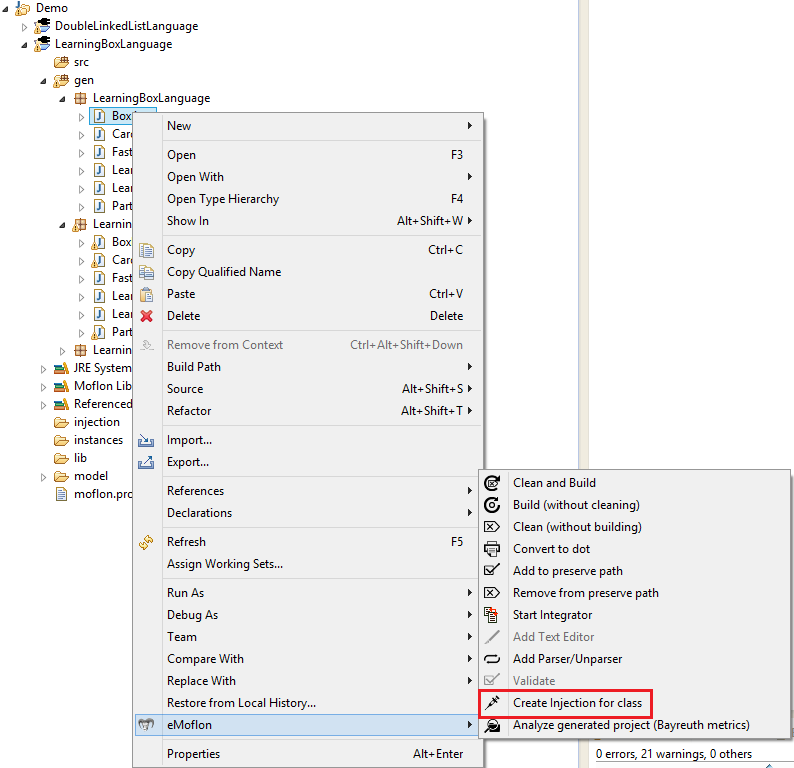
\includegraphics[width=\textwidth]{pics/injectionBilder/create_injection_context_menu.png}
        \caption{Create a new injection}
        \label{fig:injection_create_injection}
    \end{figure}

    This creates a new file in the \texttt{injection} folder of your project with the same packages and name as the Java class but with ``.inject'' as extension (Fig. \ref{fig:injection_created_injection_file}). This file contains the definition of a \textit{partial class}~(Fig.~\ref{code:generated_inject_file}) and the implementation of the method that was not specified with SDMs.

    \begin{figure}[htbp]
        \centering
        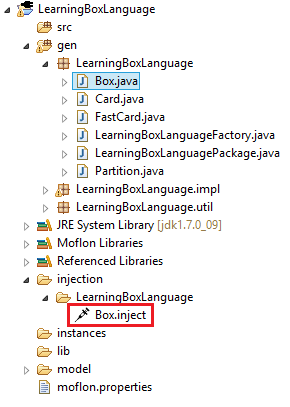
\includegraphics[width=0.54\textwidth]{pics/injectionBilder/newly_created_injection_file.png}
        \caption{Create a new injection}
        \label{fig:injection_created_injection_file}
    \end{figure}
    \FloatBarrier

    \lstdefinelanguage{Injection}[]{Java}{
        morekeywords={partial, class},
        sensitive=false,
        keywordstyle={\bfseries\color{purple}},
        emph={@model},
        emphstyle={\color{blue}},
        backgroundcolor=\color{white}
    }

    \begin{figure}[htbp]
        \centering
        \begin{lstlisting}[language=Injection]
    partial class BoxImpl {

        @model determineNextSize () <--
                // TODO: implement this method here but do not 
                // remove the injection marker
                throw new UnsupportedOperationException();
        -->

        @model addToStringRep (Card card) <--
                StringBuilder sb = new StringBuilder();

                if (stringRep == null)
                {
                    sb.append("BoxContent: [");

                }
                else
                {
                    sb.append(stringRep);
                    sb.append(", [");
                }

                sb.append(card.getFace());
                sb.append(", ");
                sb.append(card.getBack());
                sb.append("]");

                stringRep = sb.toString();
        -->

    }
        \end{lstlisting}
        \caption{Generated injection file}
        \label{code:generated_inject_file}
    \end{figure}
    \FloatBarrier

	\clearpage
    \item[$\blacktriangleright$] You now have the choice of implementing your methods directly in the injection file, or in the corresponding Java file and generating the injection from it.
    We recommend the latter as you can use the usual support from the Java editor.
    Just don't forget to update the injection before re-generating code! 
    Now complete the injection with the code given in Fig. \ref{code:complete_inject_file}.

    \begin{figure}[htbp]
        \centering
        \begin{lstlisting}[language=Injection]
partial class BoxImpl {

    @model determineNextSize () <--

            return getContainedPartition().size() * 10;
    -->

    @model addToStringRep (Card card) <--

            StringBuilder sb = new StringBuilder();

            if (stringRep == null)
            {
                sb.append("BoxContent: [");

            }
            else
            {
                sb.append(stringRep);
                sb.append(", [");
            }

            sb.append(card.getFace());
            sb.append(", ");
            sb.append(card.getBack());
            sb.append("]");

            stringRep = sb.toString();
    -->

}
        \end{lstlisting}
        \caption{Implementation of helper method as an injection}
        \label{code:complete_inject_file}
    \end{figure}
    \FloatBarrier
    \item[$\blacktriangleright$] Rebuild your project (eMoflon $\rightarrow$ Clean and build) and this code will be injected in \texttt{LearningBoxLanguage.impl.BoxImpl.java} (Fig. \ref{fig:injected_code_in_boxImpl}). For more information on injections, read \ref{sec:appendix_injections}.

\end{enumerate}



    \begin{figure}[htbp]
        \centering
        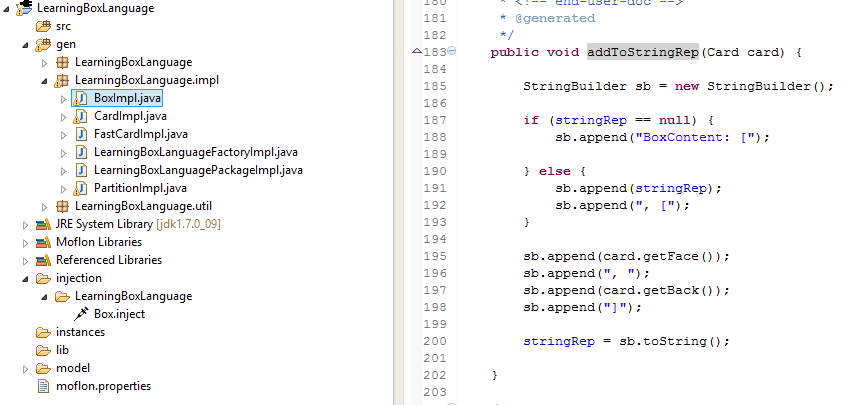
\includegraphics[angle=90,height=0.8\textheight]{pics/injectionBilder/injected_code_in_impl.png}
        \caption{Injected code in BoxImpl after code generation}
        \label{fig:injected_code_in_boxImpl}
    \end{figure}